\documentclass{standalone}
\usepackage{tikz}
\usetikzlibrary{calc}
\usetikzlibrary{decorations.markings}


\begin{document}
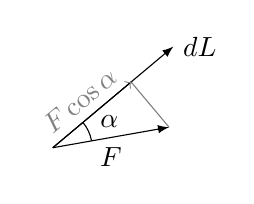
\begin{tikzpicture}[decoration={
  markings,
  mark=at position 1 with {\arrow[gray]{>}}}
]


\coordinate (O) at (0,0);
\coordinate (A) at (10:1.5);
\coordinate (B) at (40:2);

\draw[-latex] (O)--(A) node[below,pos=0.5]{$F$};
\draw[-latex] (O)--(B) node[right] {$d L$};
\draw[gray] ($(O)!(A)!(B)$)--(A);

\draw (10:0.5) arc (10:40:0.5);
\node[above right] at (16:0.5){$\alpha$};

\draw[postaction={decorate}] (O)--($(O)!(A)!(B)$) node [sloped,pos=0.5,above,gray]{$F \cos \alpha$};
\end{tikzpicture}

\end{document}
